\chapter*{Introduction} \label{chap:intr}
\addcontentsline{toc}{chapter}{Introduction}
%
%
Since the last decade, \acrfull{ai} has become increasingly part of our daily lives: chatbot, self-driving car, or playing chess are a few examples \cite{russell_artificial_2009}. \acrshort{ai} is an \textquote{umbrella term} that includes multiple approaches and a large diversity of fields such as computer vision, natural language processing, voice recognition, etc. An interesting approach of \acrshort{ai} is the ability of a machine to learn automatically. This field is called \acrfull{ml} and it has revolutionized several technology domains such as data mining, classification of new astronomical structures, etc. \cite{alom_history_2018, mitchell_machine_1997}. \textcite{mitchell_machine_1997} gives us a definition of what \acrshort{ml} is: \textquote{\textit{The concept of \acrshort{ml} relates to the question of how to construct computer programs that automatically improve with experience}}.

\textcite{arnold_introduction_2011} report that one of the challenges of traditional machine learning, given a task of interest, is the handmade selection of the most relevant features. Automatic learning of theses features using \acrfull{nn} can be used to tackle this issue. \acrfull{dl} architectures are based on this idea, composed of layers of non-linear processing. Since the previous decade, \acrshort{dl} has made breakthroughs and its fields of application have multiplied \cite{wason_deep_2018}. The accuracy of the models using this paradigm has also significantly increased. For example, in 2015, the models submitted for the image classification task achieved on average 94.5\% accuracy \cite{russakovsky_imagenet_2015}. In comparison, the submitted models for the image classification task in ILSVRC2012 achieved on average 71.3\% accuracy \cite{noauthor_imagenet_nodate}.

A type of \acrshort{dl} model, \acrfull{cnn}, demonstrates its value in applications such as image and speech processing, thanks to is high performance \cite{shawahna_fpga-based_2019}. However, the drive for improving the accuracy of such models is to increase their size, which comes at the price of a large computational and memory cost (billions of operations and millions of parameters) \cite{szegedy_going_2015, khan_survey_2020}. For example, ResNet \cite{he_deep_2016} requires 25.6M parameters and 11.3B floating-point operations for $224 \times 224$ input images.

To implement and train such computationally-intensive models, dedicated accelerators seem to be more suitable than a general \acrfull{cpu} \cite{liu_fpga-based_2019}. \acrfull{gpu}, \acrfull{asic} and \acrfull{fpga} can be used to improve the throughput and latency of \acrshort{cnn}. Today, \acrshort{cnn}s are executed on clusters of \acrshort{gpu} and \acrshort{cpu} because they provide the best throughput \cite{liu_uniform_2019}. However, they are highly demanding in terms of energy and therefore not adapted for embedded systems with constraint power resources.

For these resources constrained embedded systems, \acrshort{fpga} and \acrshort{asic} seem to be a promising solution because they are more energy-efficient. This was demonstrated by \textcite{qasaimeh_comparing_2019}. \acrshort{fpga} has a lower energy consumption compared to \acrshort{gpu} by several orders of magnitude, as the vision application’s pipeline complexity grows (which is the case for \acrshort{cnn}). We can observe in Table \ref{tab:benchener} the FPGA’s energy reduction ratios to GPU for various vision application’s pipelines. Moreover, because the \acrshort{fpga} has the property of reconfigurability comparing to the \acrshort{asic}, developing accelerators on \acrshort{fpga} is time and cost-effective \cite{motamedi_placid_2017}. Therefore, \acrshort{fpga} should be the platform to run \acrshort{cnn} on mobile devices.
%
\begin{table}[H]
    \center
    \begin{tabular}{|c|c|}
        \hline
        Pipeline & Energy/frame (mJ/f) \\
        \hline
        Background Subtraction & 1.74 $\times$\\
        \hline
        Color Segmentation & 1.86 $\times$ \\
        \hline
        Harris Corners Tracking & 3.94 $\times$ \\
        \hline
        Stereo Block Matching & 8.83 $\times$ \\
        \hline
    \end{tabular}
    \caption{FPGA’s Reduction Ratios to GPU, from \cite{qasaimeh_comparing_2019}}
    \label{tab:benchener}
\end{table}

Furthermore, while \acrshort{gpu} is currently the most dominant platform to perform \acrshort{cnn}s, trends confirm that \acrshort{fpga} will be more suitable to accelerate them, according to \textcite{nurvitadhi_can_2017}. Two reasons can explain that. First, the advances in \acrshort{fpga} technology show that the performance disparity between \acrshort{fpga} and \acrshort{gpu} has lessened. Second, recent \acrshort{cnn} trends use pruning and extremely quantized data types to reduce the size of the \acrshort{cnn}. It is in favor of the \acrshort{fpga} because those two approaches are easier to handle on it. However, \acrshort{fpga} is resource-constraint (limited memory, I/O bandwidth, and computing resources). As a result, the challenge is to find a mapping between the computational and the execution model \cite{morcel_feathernet_2019}.

According to \textcite{abdelouahab_accelerating_2018}, there are 2 phases when executing a \acrshort{cnn}. The first phase is the \textbf{training}, where the model learns using the back-propagation algorithm \cite{lecun_backpropagation_1989}. The second phase is the \textbf{inference}, where the model predicts the output of new data samples, using the learned model and the feed-forward algorithm \cite{zhang_optimizing_2015}. We can see the different processes in Figure \ref{fig:traininf}. Usually, \acrshort{cnn}s are trained once on \acrshort{gpu} or \acrshort{fpga} and inference is executed every time \acrshort{cnn} has to process new input. So, most efforts need to be focused on accelerating the inference phase \cite{abdelouahab_accelerating_2018}. The core of this work is therefore aimed at proposing a way to accelerate the inference of a model on \acrshort{fpga}.
%
\begin{figure}[H]
    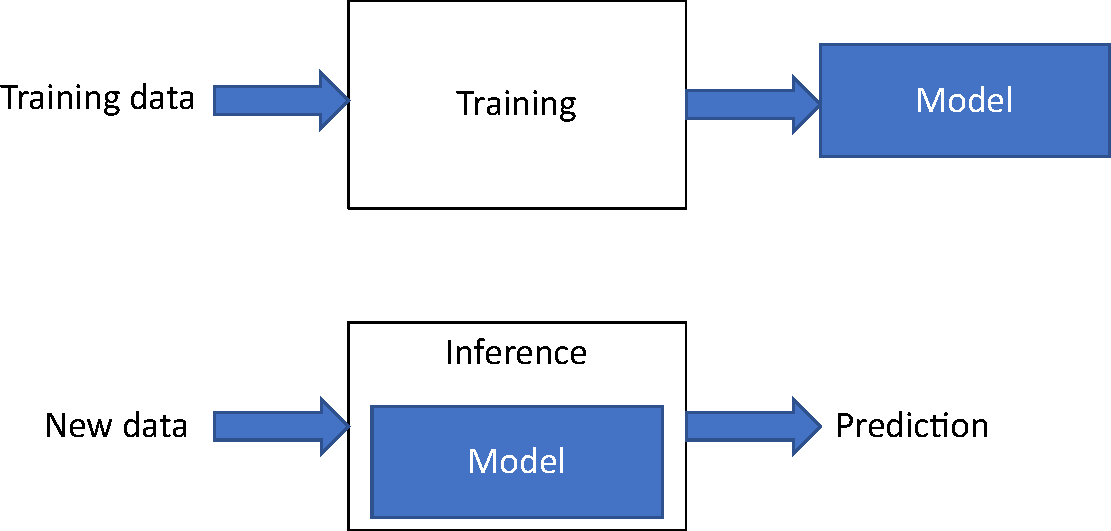
\includegraphics[width=\textwidth]{traininf.pdf}
    \caption{\acrshort{cnn} execution phases, inspired by \cite{nurvitadhi_can_2017}}
    \label{fig:traininf}
\end{figure}

The inference can be accelerated using various optimizations. According to \textcite{abdelouahab_accelerating_2018}, these optimizations can be grouped into 3 main categories:
\begin{itemize}
    \item \textbf{Algorithmic Optimizations}: the computational complexity of \acrshort{cnn}s can be reduced by vectorizing the operations or using faster algorithms.
    \item \textbf{Datapath Optimization}: because of the limited resources on an FPGA, memory is often the bottleneck, and optimizing the memory management can increase the throughput.
    \item \textbf{\acrshort{cnn} model Optimization}: an important issue of \acrshort{cnn} is their computational complexity and hardware utilization. A solution is to trade accuracy for acceleration by using approximate computing.
\end{itemize}

\textbf{\acrshort{cnn} model Optimization} is going to be the key point of this work because the \acrshort{cnn} size and arithmetic complexity are the major issues when implementing a \acrshort{cnn} on mobile devices \cite{cheng_recent_2018}. One of these optimizations, named weights pruning, consists of removing all unnecessary weights of the network \cite{abdelouahab_accelerating_2018}.

This work focus on weights pruning. The irregular data access and the custom data type of the non-pruned weights show it is suitable to implement pruning on \acrshort{fpga}. Therefore, this work concentrates on building an architecture using pruning on \acrfull{dsc}, an alternative way to perform convolution which uses fewer parameters and has a lesser computational complexity. The objective of this work is then to build an efficient architecture on \acrshort{fpga} implementing a sparse \acrshort{cnn} network using \acrshort{dsc}. To assess the benefits of the proposed pruning, we have chosen MobileNetV2 because it offers state of the art performance \cite{sandler_mobilenetv2_2018}.

These work achievements are the following:
%
\begin{itemize}
    \item A structured pruning scheme is proposed to reduce the number of parameters and the computational complexity of the \acrshort{dsc}.
    \item To reduce memory usage, a compressed format is developed to store the non-pruned weights.
    \item An accelerator is designed to support the MobileNetV2 building block performing the sparse \acrshort{dsc}.
    \item The obtained results show that the structured pruning scheme allows a reduction of the computational complexity and the number of parameters, and a faster inference by reducing the latency to execute the \acrshort{dsc}.
\end{itemize}
%
%
\section*{Structure of the thesis}
\addcontentsline{toc}{section}{Structure of the thesis}
%
%
This master thesis is composed of 3 chapters.

Chapter \ref{chap:background} details the background information about the two main topics of this thesis: \acrshort{cnn} and \acrshort{fpga}. First, we explore the theory behind \acrshort{cnn} and go deeper into its computational background in Section \ref{sec:cnn}. Then, the concept and workflow of \acrshort{fpga} are explained in Section \ref{sec:fpga}.

Using knowledge of Chapter \ref{chap:background}, we explore in Chapter \ref{chap:sota} the state of the art techniques on accelerating the inference on \acrshort{fpga}. We explore algorithmic and model optimizations to reduce the cost of the convolution operation and the size of the models. The chapter also details datapath optimizations which reduce the inefficiency of the convolution on \acrshort{fpga}. We also review various \acrshort{fpga} architectures implementing \acrshort{dsc} and pruning of standard convolution.

Chapter \ref{chap:pratique} uses the knowledge from Chapter \ref{chap:sota} to design an efficient architecture using pruning and depthwise separable convolution. It also details the experimental setup to measure the performance of the developed architecture and discusses the obtained results

Finally, a conclusion on this work and the obtained results are done in the Conclusion. A discussion on the methodology and future works is also presented.

\afterpage{\blankpage}
\cleardoublepage
\newpage
